\documentclass[mathserif]{beamer}
\usepackage{amsmath}
\mode<presentation>
\usetheme{Madrid}
\AtBeginSection[]{}
\title{Phase Transitions and Scale Free Phenomena in Networks of Memristive Elements}
\author{Forrest Sheldon}
\date{August 7, 2015}
\titlegraphic{
\includegraphics[width=2.5cm]{gl-1-logo.png}}
\begin{document}

\begin{frame}
\titlepage
\end{frame}

\begin{frame}
\frametitle{A Perspective On Memristors}

\begin{columns}
\column{0.5\textwidth}
\begin{itemize}
\item Simple(est) Nanomachines
\item Sit between scales
\item Wide variety of behaviors: ON/OFF ratio, volatility, timescales, programmability

\end{itemize}
\column{0.5\textwidth}
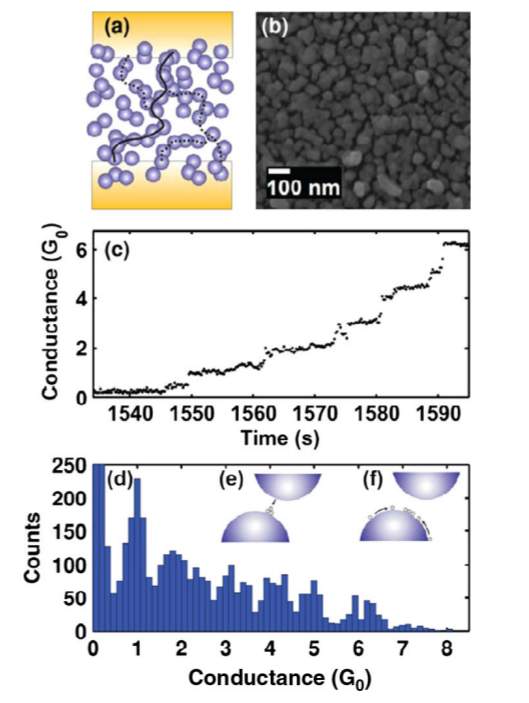
\includegraphics[width=5cm]{Granular_Material.png}
\end{columns}
\end{frame}

\begin{frame}
\frametitle{Example: $Ag|Ag_2 S|Ag$ Atomic Switch}
\begin{center}
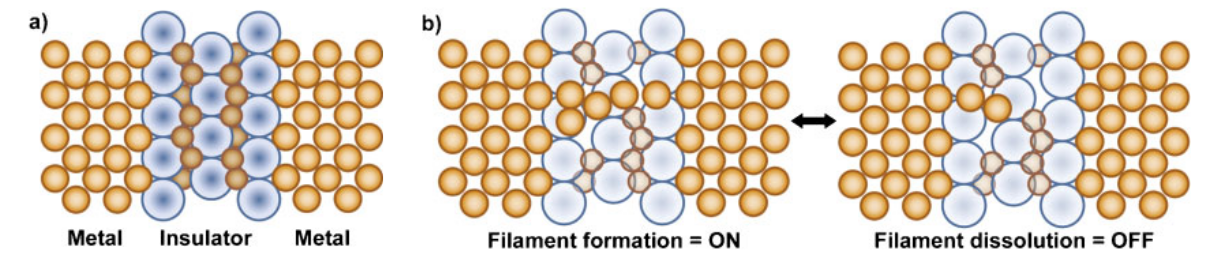
\includegraphics[width=10cm]{Atomic_Switch_Filament.png}
\end{center}
\begin{itemize}
\item Rely on Ionic motion
\item Strong threshold effect from competition between thermal effects and filament formation
\item Device Size $\approx 100$nm, Switching Times $~10^{-7}$s or less
\item Dynamics allow them to show short term and long term potentiation-like behaviors,
operating in stochastic and non-volatile regimes, and can store multiple states in quantized conductance

\end{itemize}
\end{frame}

\begin{frame}
\frametitle{Memristor Network}


\end{frame}

\begin{frame}
\frametitle{Length and Time Scales}


\end{frame}

\begin{frame}
\frametitle{Memristor Model}
Memristors show a super exponential change in their state - switching past
this threshold is extremely quick in comparison to the external voltage.  As such,
we choose a model in which the memristors switch instantly once the threshold has
been crossed
\end{frame}

\begin{frame}
\frametitle{One-Dimensional Models}
Parallel doesn't work.


\end{frame}



\end{document}
